\subsection{The glass transition}

\begin{frame}{The glass transition}
	\begin{columns}
	\column{0.6\textwidth}
	\resizebox{1.1\columnwidth}{!}{\input{cooling.pdf_tex}}%\\
	%\begin{footnotesize}\citet{cavagna2009supercooled}\end{footnotesize}
	\column{0.4\textwidth}
	\begin{itemize}
		\item Avoid crystallisation
		\item Slowing down by orders of magnitude
		\item A different type of solid: Glass
	\end{itemize}
	\end{columns}
	\begin{itemize}
		\item Kinetic glass transition $T_g$
		\item Not a thermodynamic transition but a dynamical arrest
	\end{itemize}
\end{frame}

\begin{frame}{Glass are amorphous}
	\begin{columns}
	\column{0.5\textwidth}
	Static structure factor
	\centering
	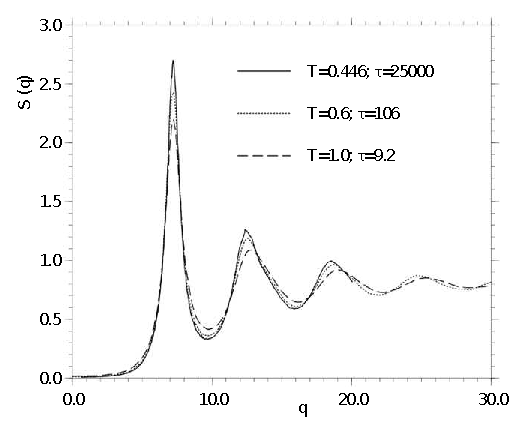
\includegraphics[width=\columnwidth]{sq_kob}
	
	\footnotesize{\citet{Kob2002}}
	
	\column{0.5\textwidth}
	While dynamics changes by 4 orders of magnitude
	\begin{itemize}
		\item Almost no change in positional order
		\item No characteristic length scale diverging toward $T_g$ or $T_0$
		\item $\neq$ critical phenomena
	\end{itemize}
	\end{columns}
\end{frame}

\begin{frame}{Fragility: super-Arrhenius behaviour}
	\begin{columns}
	\column{0.6\textwidth}
	\centering
	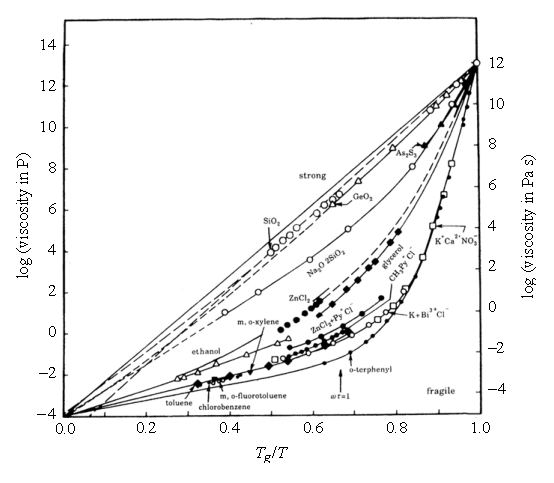
\includegraphics[width=\columnwidth]{angell}
	
	\footnotesize{\bibentry{ANGELL1988}}
	
	\column{0.4\textwidth}
	Vogel-Fulcher-Tamman empirical law:
	\[ 
	\tau = \tau_0 \exp{\left(\mathcal{D}\frac{T_0}{T_0-T}\right)}
	\]
	\begin{description}
		\setlength{\itemindent}{-4em}
		\item[$T_0$] "ideal" glass transition temperature
		\item[$\mathcal{D}$] fragility
	\end{description}
	
	\end{columns}
\end{frame}

\subsection{Dynamics of supercooled liquids}

\begin{frame}{Two step relaxation}
	\begin{columns}
	\column{0.5\textwidth}
	Self intermediate scattering function:
	\centering
	\def\svgwidth{\columnwidth}\input{isf_kob.pdf_tex}\\
	\footnotesize{\bibentry{Kob1995}}
	
	\column{0.5\textwidth}
	Supercooled liquid is ergodic
	\begin{itemize}
		\item A plateau appear
		\item $\beta$-relaxation does not change
		\item The length of the plateau changes\\ $\Rightarrow$ slowing down by many orders of magnitude
	\end{itemize}
	\end{columns}
\end{frame}

\begin{frame}{The cage theory}
	\begin{columns}
	\column{0.5\textwidth}
	\centering
	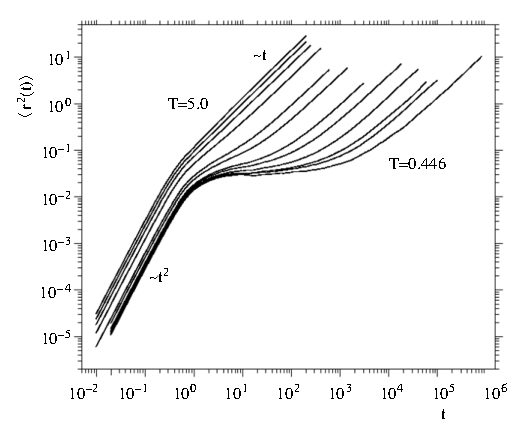
\includegraphics[width=\columnwidth]{msd_kob}
	
	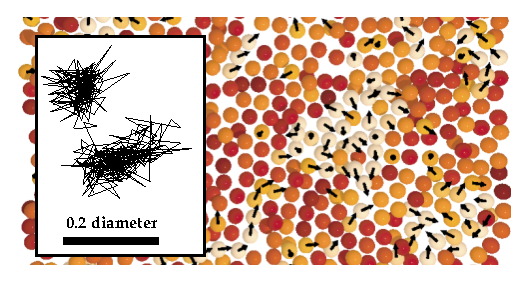
\includegraphics[width=\columnwidth]{cage_weeks}
	
	\column{0.5\textwidth}
	Mean square displacement\\
	\begin{footnotesize}\bibentry{kob1995tmc}\end{footnotesize}
	
	\bigskip
	\begin{itemize}
		\item Hopping between cages $\ll\sigma$
		\item Is the hopping probability really uniform?
	\end{itemize}
	
	\bigskip
	\begin{footnotesize}\bibentry{weeks2002pcr}\end{footnotesize}
	\end{columns}
\end{frame}

\begin{frame}{Dynamic heterogeneities}
	Fast and slow regions exist at intermediate times.
	\begin{columns}[t]
	\column{0.5\textwidth}
	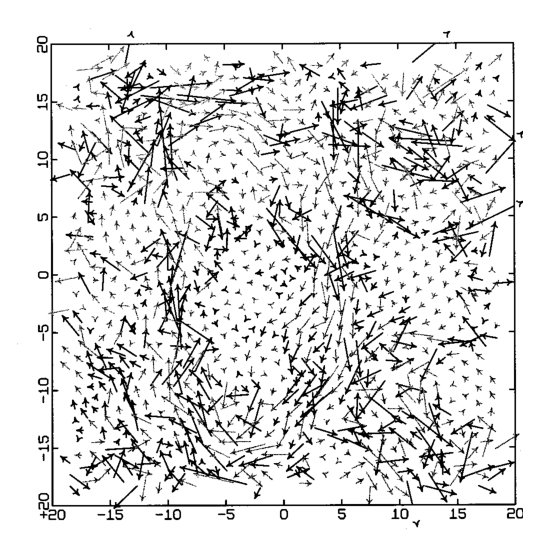
\includegraphics[width=\columnwidth]{dh_perera}
	\column{0.5\textwidth}
	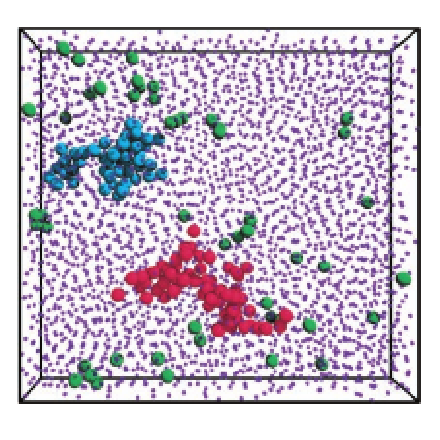
\includegraphics[width=\columnwidth]{dh_weeks}\\
	\centering{$10\%$ fastest particles}
	\end{columns}
	
	\bigskip
	\begin{footnotesize}
	\begin{columns}
	\column{0.5\textwidth}
	\bibentry{Perera1999}
	\column{0.5\textwidth}
	\bibentry{weeks2000}
	\end{columns}
	\end{footnotesize}
\end{frame}

\begin{frame}{Dynamical length scale}
	\begin{columns}
	\column{0.5\textwidth}
	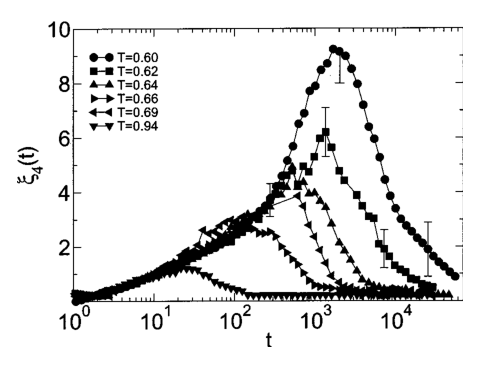
\includegraphics[width=\columnwidth]{xi4_lacevic}\\
	\begin{footnotesize}\centering\citet{Lacevic2003}\end{footnotesize}
	\column{0.5\textwidth}
	\begin{itemize}
	\item Spatial correlation of the fluctuations of the dynamics.
	\item Extract a dynamical correlation length
	\item Grows toward the glass transition
	\end{itemize}
	\end{columns}
	\begin{center}
	No statical length scale opens the door to exotic physics	
	\begin{itemize}
		\item Facilitation
		\item Space-time thermodynamics
		\item $\dots$
	\end{itemize}
	\end{center}
\end{frame}

\subsection{Quest for a static explanation?}
\begin{frame}{Static cause to dynamic heterogeneities}
	\begin{columns}
	\column{0.5\textwidth}
	\centering
	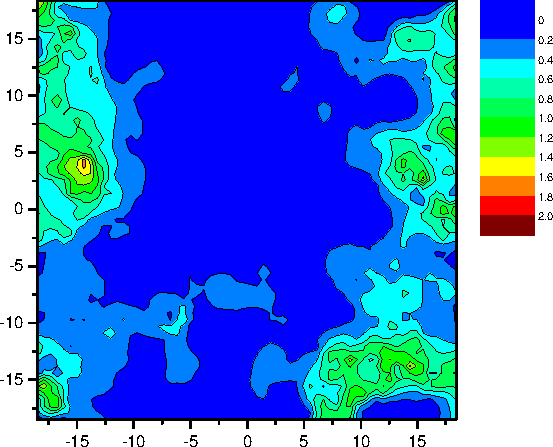
\includegraphics[width=\columnwidth]{propensity}
	\column{0.5\textwidth}
	\footnotesize{\citet{Widmer-Cooper2005}}
	\begin{itemize}
		\item $N$ runs from the same initial configuration
		\item Average out the influence of initial dynamics
		\item Propensity to displacement
		\item Predict fast/slow \alert{regions} \footnotesize{\citep{Berthier2007}}
	\end{itemize}
	\end{columns}
	
	\bigskip$\Rightarrow$ Glass transition may have a structural cause
\end{frame}

\begin{frame}{Structural cause}
	\begin{columns}
	\column{0.3\textwidth}
	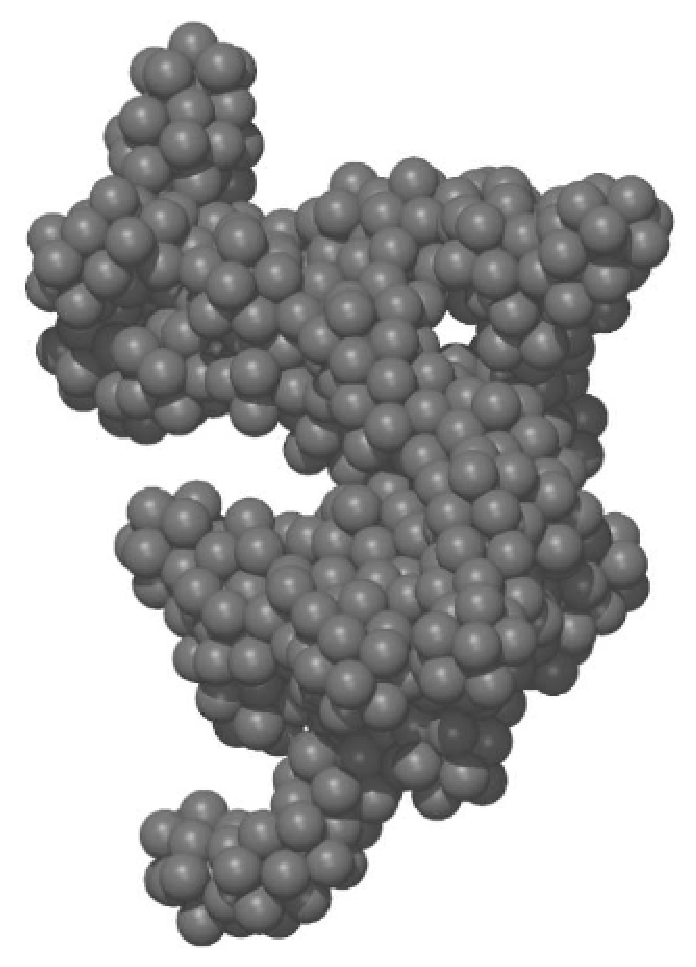
\includegraphics[width=\columnwidth]{Dzugutov_LFS}\\
	\begin{footnotesize}\citet{Dzugutov2002}\end{footnotesize}
	\column{0.5\textwidth}
	\citet{tarjus2005fba}
	\begin{itemize}
		\item Locally favoured structures
		\item Cannot fill space because of \alert{frustration}
		\item The ground state exist in
		\begin{itemize}
			\item Curved space
			\item 4 dimensions
		\end{itemize}
		\item LFS are slow		
	\end{itemize}
	\end{columns}
\end{frame}

\begin{frame}{Structural cause}
	\begin{footnotesize}\citet{tanaka2010critical}\end{footnotesize}
	\begin{columns}
	\column{0.33\textwidth}\centering
	\resizebox{\columnwidth}{!}{\input{kawa_nm_psi6.pdf_tex}}\\
	$\Psi_6$
	\column{0.33\textwidth}\centering
	\resizebox{\columnwidth}{!}{\input{kawa_nm_msd.pdf_tex}}\\
	$\Delta r^2$
	\end{columns}
	\begin{itemize}
		\item The ground state is the crystal
		\item Frustration \alert{against} crystallisation
		\begin{itemize}
			\item Other structures are locally more stable
			\item Polydispersity
		\end{itemize}
		\item Slowing down $\Leftrightarrow$ local crystal-like order
	\end{itemize}
\end{frame}

\begin{frame}{Purpose}
	\begin{itemize}
		\item Unified picture of the glass transition
		\item Quest for a static (structural) length scale diverging toward $\phi_0$
	\end{itemize}
	
	\bigskip In hard sphere colloidal supercooled liquid
	\begin{itemize}
		\item Which structure(s) is/are linked with dynamic heterogeneities?
		\item What are the relevant structures?
	\end{itemize}
\end{frame}
